%%%%%%%%%%%%%%%%%%%%%%%%%%%%%%%%%%%%%%%%%%%%%%%%%%%%%%%%%%%%
%%  This Beamer template was created by Cameron Bracken.
%%  Anyone can freely use or modify it for any purpose
%%  without attribution.
%%
%%  Last Modified: January 9, 2009
%%

\documentclass[xcolor=x11names,compress]{beamer}
\usepackage[utf8]{inputenc} 
\usepackage[T1]{fontenc}
\usepackage{cmbright}

%% General document %%%%%%%%%%%%%%%%%%%%%%%%%%%%%%%%%%
\usepackage{graphicx}
\usepackage{caption}  
\usepackage{subcaption}     % subfloats


\usepackage{tikz}

\usepackage[style=authoryear]{biblatex}
\usetikzlibrary{decorations.fractals}
%%%%%%%%%%%%%%%%%%%%%%%%%%%%%%%%%%%%%%%%%%%%%%%%%%%%%%


%% Beamer Layout %%%%%%%%%%%%%%%%%%%%%%%%%%%%%%%%%%
\useoutertheme[subsection=false,shadow]{miniframes}
\setbeamerfont{title like}{shape=\scshape}
\setbeamerfont{frametitle}{shape=\scshape}

\setbeamercolor*{lower separation line head}{bg=DeepSkyBlue4} 
\setbeamercolor*{normal text}{fg=black,bg=white} 
\setbeamercolor*{alerted text}{fg=red} 
\setbeamercolor*{example text}{fg=black} 
\setbeamercolor*{structure}{fg=black} 

\usenavigationsymbolstemplate{}
\setbeamercolor*{palette tertiary}{fg=black,bg=black!10} 
\setbeamercolor*{palette quaternary}{fg=black,bg=black!10} 

\setbeamercovered{dynamic} % enable pause

\renewcommand{\(}{\begin{columns}}
\renewcommand{\)}{\end{columns}}
\newcommand{\<}[1]{\begin{column}{#1}}
\renewcommand{\>}{\end{column}}
%%%%%%%%%%%%%%%%%%%%%%%%%%%%%%%%%%%%%%%%%%%%%%%%%%
\useoutertheme{infolines} % authors, etc.
%%%%%%%%%%%%%%%%%%%%%%%%%%%%%%%%%%%%%%%%%%%%%%%%%%

\bibliography{presentation.bib}

\DeclareGraphicsExtensions{.pdf,.png,.jpg, .eps}

\usepackage{color, colortbl}  
\definecolor{LightCyan}{rgb}{0.88,0.8,1}
\begin{document}


\begin{frame}{}
\title[Neocortex]{A network model of the neocortex}
\author{
Friedrich Schüßler}
\date{\today}
\titlepage

\centering 
Supervisor: Prof. Stefan Rotter \& Benjamin Merkt
\end{frame}

\begin{frame}{Table of contents}
    \tableofcontents
\end{frame}

\AtBeginSection[]{
\begin{frame}{Table of contents}
    \tableofcontents[currentsection]
\end{frame}
}


%\section{Intro}
%\begin{frame}[t]{Introduction}
%\begin{itemize}
%    \item Local cortical network is structure in layers
%    \item Relationship between structure and activity poorly understood
%    \item Experimental data only partly reproduced
%    \item Potjans assembles connectivity map in 2012
%\end{itemize}
%\end{frame}
%

\section{Network model}
\begin{frame}[t]{Layered structure}
\begin{figure}[htpb]
    \centering
    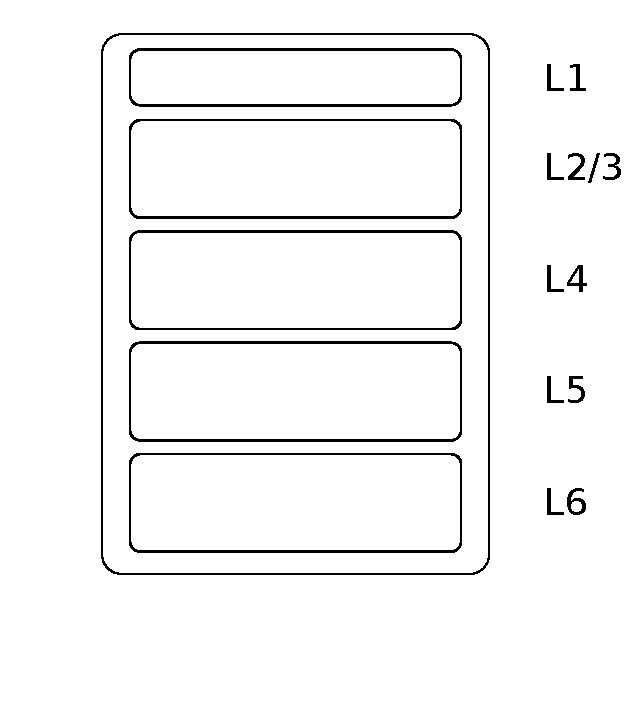
\includegraphics[width=0.5\linewidth]{../figures/microcircuit_model_pre}
\label{fig:model_0}
\end{figure}
\end{frame}

\begin{frame}[t]{Layered structure}
\begin{figure}[htpb]
    \centering
    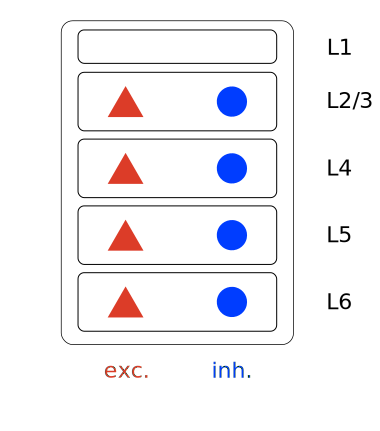
\includegraphics[width=0.5\linewidth]{../figures/microcircuit_model_pre0}
\label{fig:model_1}
\end{figure}
\end{frame}

\begin{frame}[t]{Layered structure}
\begin{figure}[htpb]
    \centering
    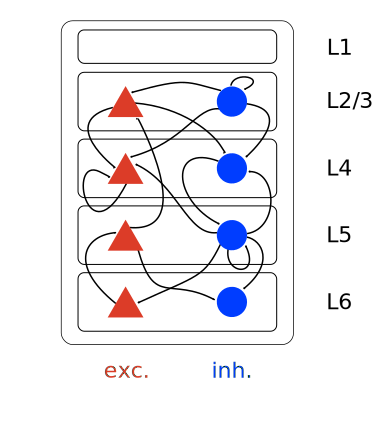
\includegraphics[width=0.5\linewidth]{../figures/microcircuit_model_pre1}
\label{fig:model_2}
\end{figure}
\end{frame}

\begin{frame}[t]{Layered structure}
\begin{figure}[htpb]
    \centering
    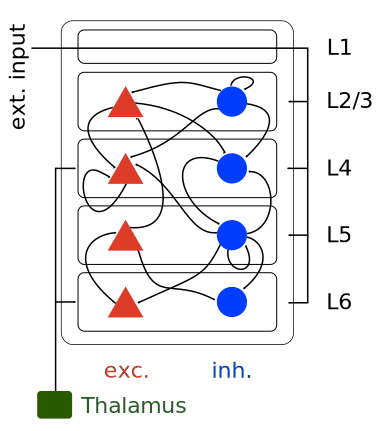
\includegraphics[width=0.5\linewidth]{../figures/microcircuit_model_full}
\label{fig:model3}
\end{figure}
\end{frame}

\begin{frame}[t]{Network parameters}
\begin{table}[htpb]
    \centering
    \label{tab:network_parameters}
    \begin{tabular}{l l}
        \rowcolor{LightCyan} Parameter specification & \\
        \cellcolor{LightCyan} Total population size & $\approx 80,000$\\
        \cellcolor{LightCyan} Total synapse number  & $\approx 0.3 \cdot 10^9$\\
        \cellcolor{LightCyan} Neuron model          & Leaky integrate-and-fire\\
        \cellcolor{LightCyan} Synapse model         & Exponential-shaped postsynaptic currents\\
        \cellcolor{LightCyan} Rel. inh. synaptic strength & $g = -4.0$\\
    \end{tabular}
\end{table}
\end{frame}

\begin{frame}[t]{Network parameters}
\begin{figure}
    \centering
    \begin{subfigure}[b]{0.31\textwidth}
        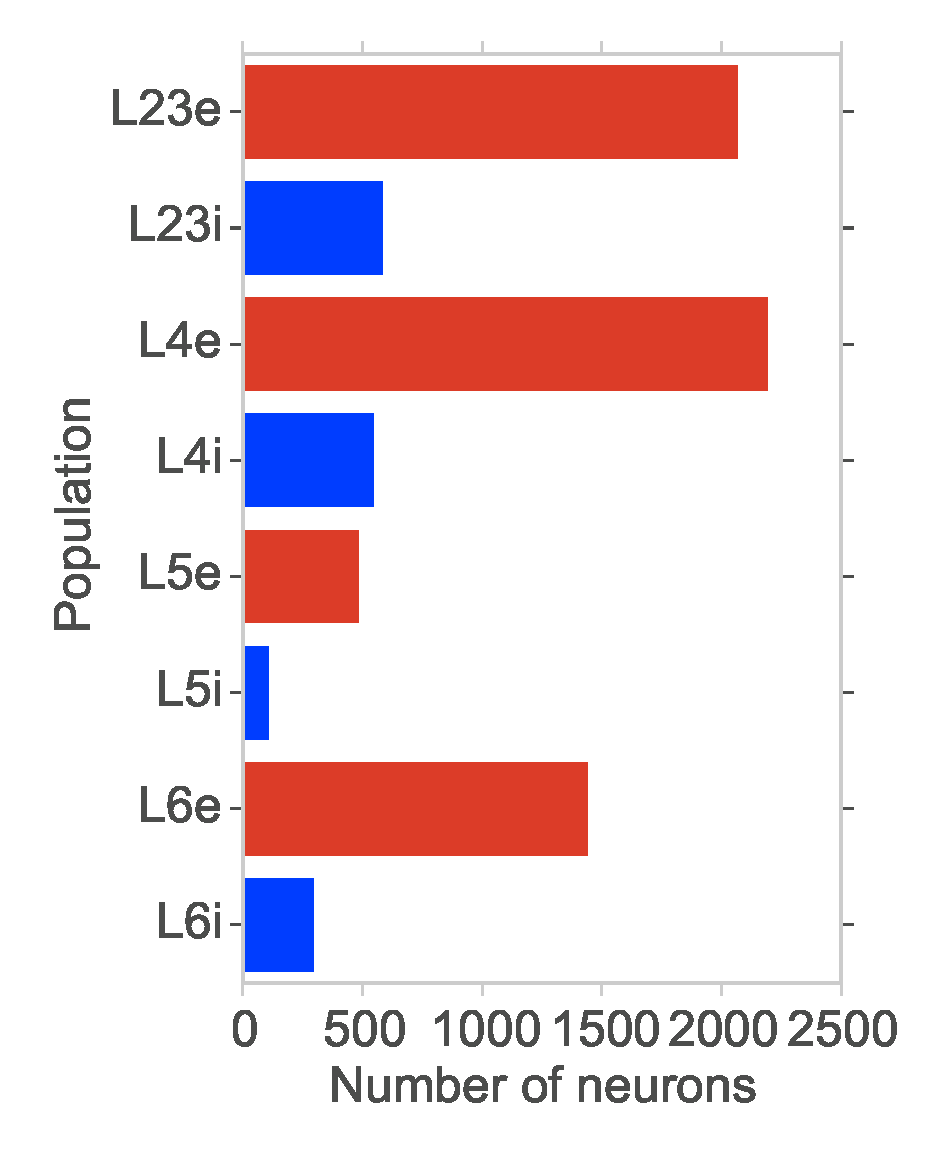
\includegraphics[width=\textwidth]{../figures/population_sizes}
        \caption{Population size}
        \label{fig:pop_size}
    \end{subfigure}
    \quad
    \begin{subfigure}[b]{0.64\textwidth}
        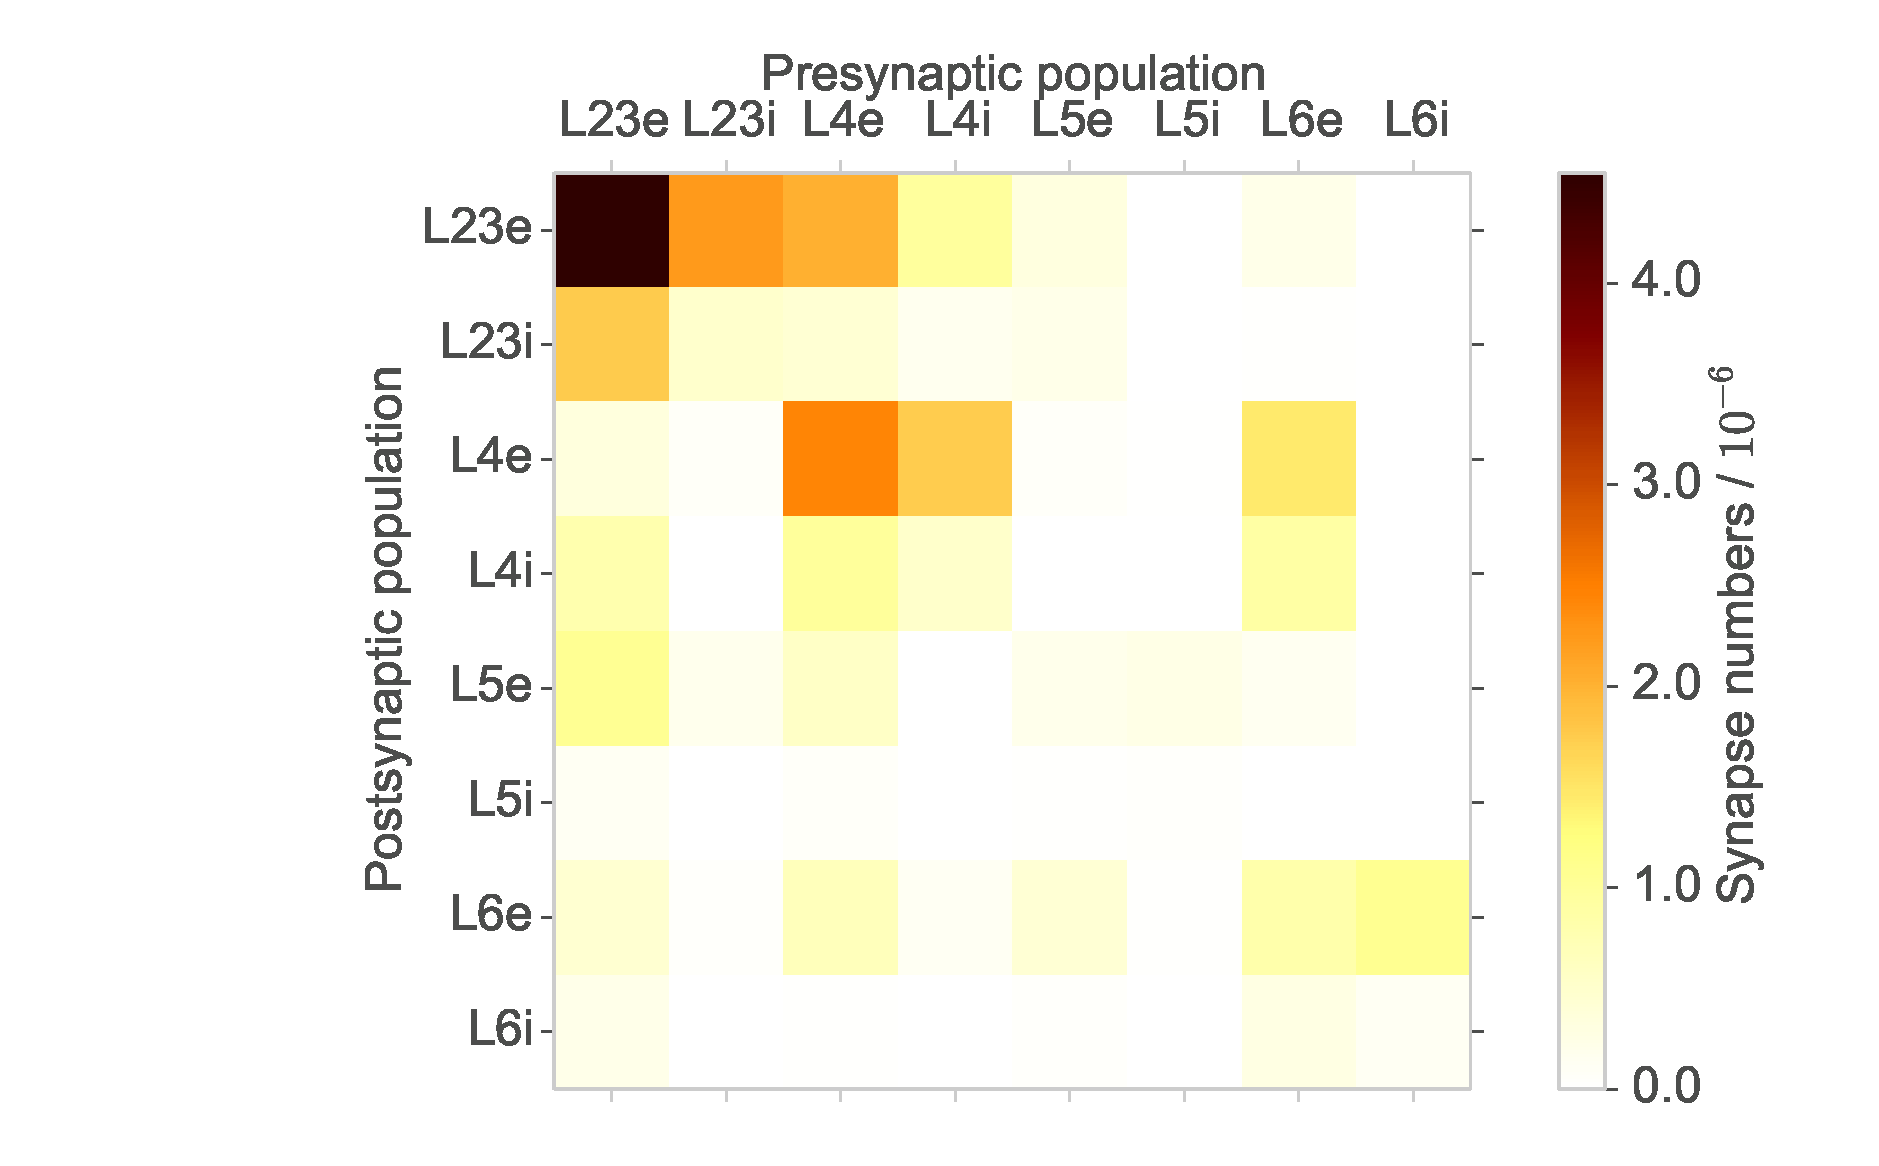
\includegraphics[width=\textwidth]{../figures/heat_map_syn_numbers}
        \caption{Synapse numbers}
        \label{fig:syn_numbers}
    \end{subfigure}
\end{figure}
\end{frame}

%\begin{frame}[t]{Connection probabilities}
%\begin{figure}[htpb]
%    \centering
%    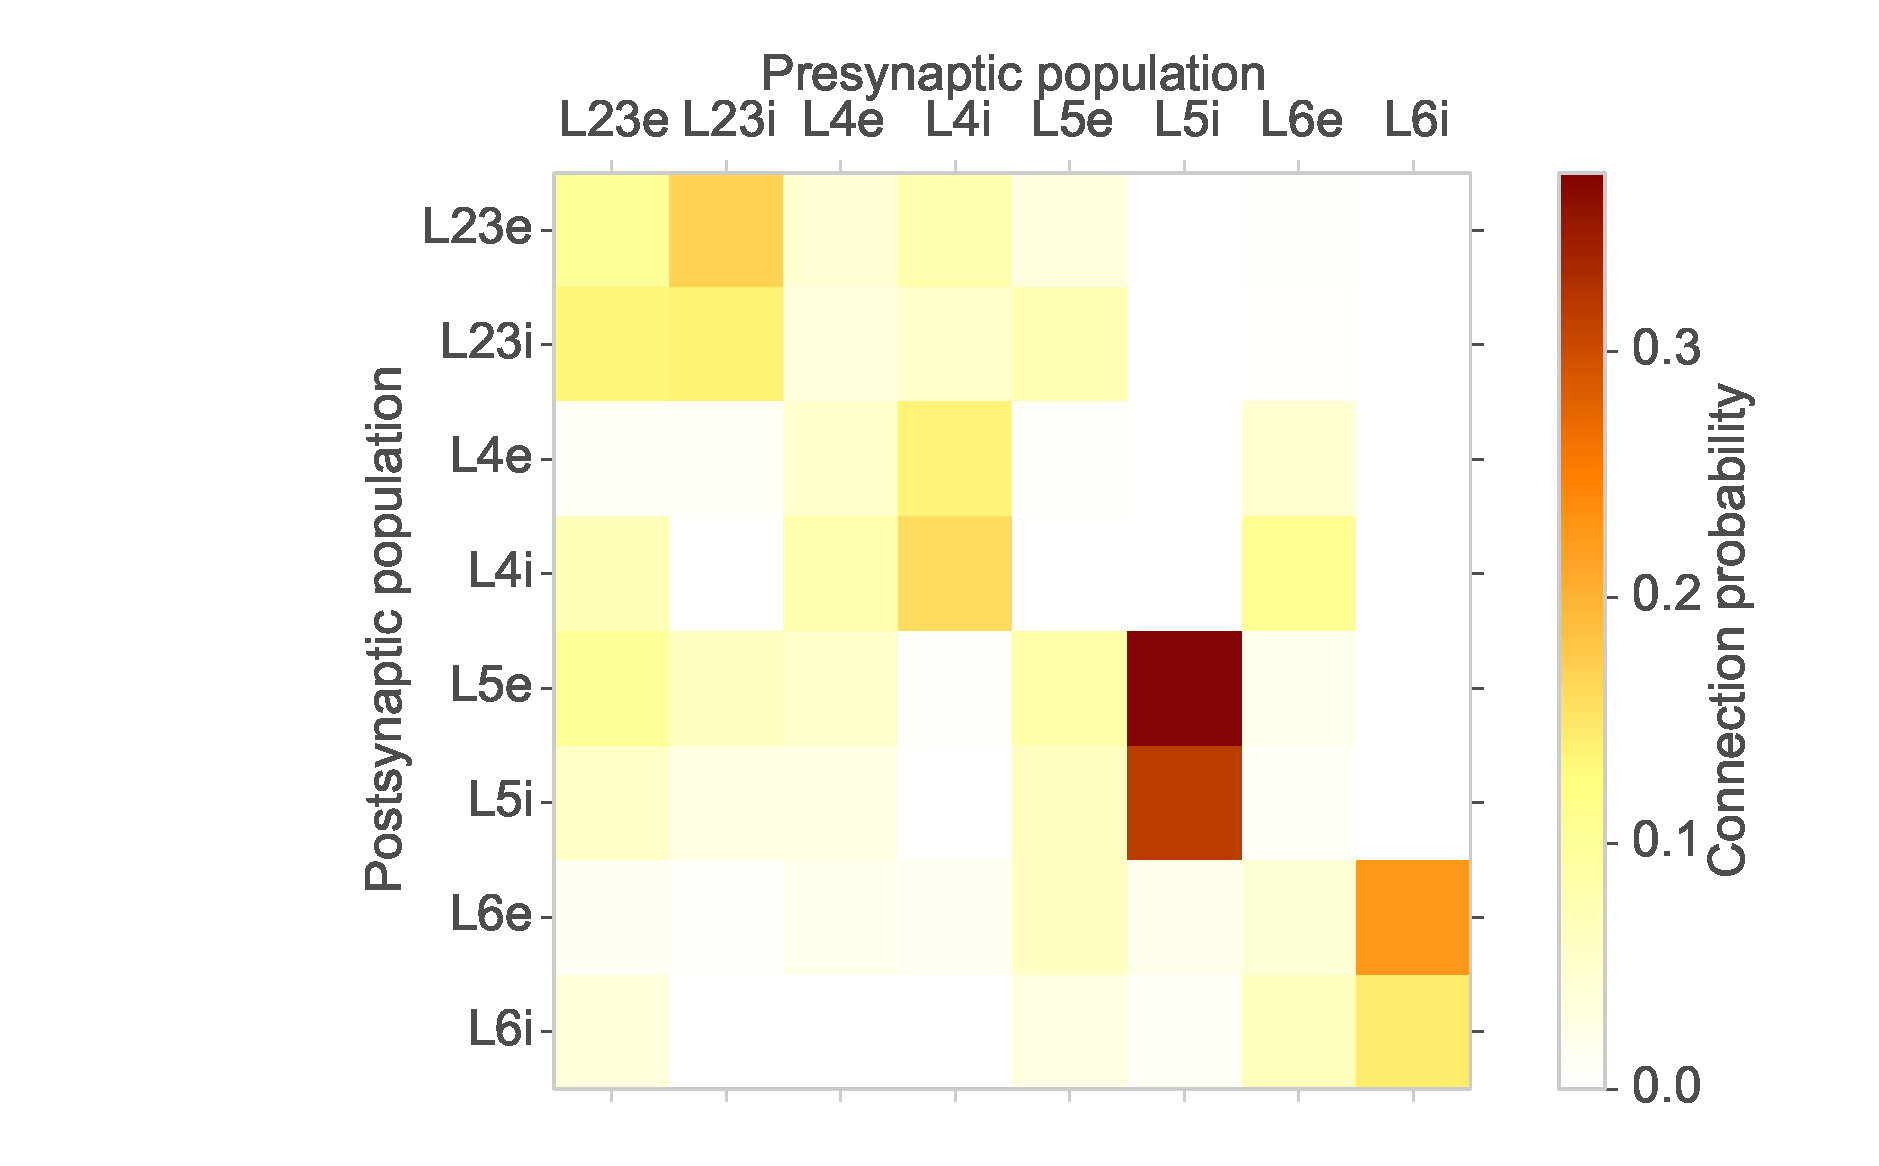
\includegraphics[width=0.9\linewidth]{../figures/heat_map_conn_probs}
%\label{fig:conn_probs}
%\end{figure}
%\end{frame}
%

\section{Mean field model}
\begin{frame}[t]{Neuron depolarization}
Membrane potential $V_i$ at timescale $\tau$ follows
\begin{equation}
    \tau \dot{V_i}(t) = -V_i(t) + R I_i(t) \, .
    \label{depol} 
\end{equation}
The model goes from a deterministic description,
\begin{align}
    R I_i(t)    &= \tau \sum_j J_{ij} \sum_k \delta(t - t_j^k - D) 
    \label{input_det}
\intertext{to a statistical one:}
    R I_i(t)   &= \mu(t) + \sigma(t) \sqrt{\tau} \eta_i(t) 
    \label{input}
\end{align}
Here, $\eta_i(t)$ is uncorrelated gaussian white noise.
\end{frame}

\begin{frame}[t]{Self-consistent solution in 2D model}
Firing rate $\nu$ of each neuron obeys
\begin{equation}
    \frac{1}{\nu} = \tau_{rp} + 
        2 \, \tau \int_{\frac{V_r - \mu}{\sigma}}^{\frac{\theta - \mu}{\sigma}} 
        e^{u^2} \left(1 + \text{erf}(u)\right) \,\text{d}u 
\end{equation}
with average input
\begin{align}
    \mu        &= 
        \tau C \, J \,\left(1 - \gamma g \right) \nu \quad
        + 
        \tau C \, J \, \nu_{ext} \\
\intertext{and fluctuations}
    {\sigma}^2 &=
        \underbrace{
            \tau C \, J^2 \left(1 + \gamma g^2\right) \, \nu
        }_\text{local} +
        \underbrace{
            \tau C \, J^2 \,\nu_{ext} 
        }_\text{external} \,.
\end{align}
\end{frame}

\begin{frame}[t]{Goals}
\begin{enumerate}
    \visible<1-|handout:0>{\item Reconstruct the original model in \emph{pynest}
    \vfill
    }
    \visible<2-|handout:0>{\item Develop a mean field model for firing rates
    \vfill
    }
    \visible<3>{\item Compare network model with mean field model
    }
\end{enumerate}
\end{frame}

%\begin{frame}[t]{Goals}
%\begin{enumerate}
%    \item On the original model
%    \begin{itemize}
%        \item Reconstruct the model in \emph{pynest}
%        \item Verify the equality of both implementations
%        \item Allow to easily extend the model to more neuron types
%        \item Test statistical robustness
%    \end{itemize}
%    \item Developing a mean field model
%    \begin{itemize}
%        \item Extend Brunel's model to 8 dimensions
%        \item Calculate firing rates for parameters as in Potjans' model
%        \item Where and why does the mean field model fail?
%    \end{itemize}
%    \item Compare both models
%    \begin{itemize}
%        \item Simulate parallel to numerical solving
%        \item Test robustness on various parameters:
%        \begin{itemize}
%            \item neuron numbers
%            \item synapse numbers (fixed?)
%            \item distributions for weights and delays
%        \end{itemize}
%    \end{itemize}
%\end{enumerate}
%\end{frame}
%

\section{Preliminary results}
\begin{frame}[t]{Compare SLI and pynest implementations}
\begin{figure}
    \centering
    \visible<1-|handout:0>{
    \begin{subfigure}[b]{0.40\textwidth}
        \includegraphics[width=\textwidth]{../../analysis/figures/{{spon_activity_a1.0_t20.0_00_sli}}}
        \caption{SLI}
        \label{fig:sim_pynest}
    \end{subfigure}
    \quad
    }
    \visible<2>{
    \begin{subfigure}[b]{0.40\textwidth}
        \includegraphics[width=\textwidth]{../../analysis/figures/{{spon_activity_a1.0_t20.0_00}}}
        \caption{Pynest}
        \label{fig:sim_pynest}
    \end{subfigure}
    }\par
\end{figure}
\end{frame}

%\begin{frame}[t]{Membrane potential distribution}
%\begin{figure}[htpb]
%    \centering
%    \includegraphics[width=0.9\textwidth]{../../analysis/figures/{{membrane_potential_a1.0_t20.0_00_L23e}}}
%    \label{fig:pop_size}
%\end{figure}
%\end{frame}
%
\begin{frame}[t]{Membrane potential distribution}
\begin{figure}[htpb]
    \centering
    \includegraphics[width=0.9\textwidth]{../../analysis/figures/{{membrane_potential_a1.0_t20.0_00}}}
    \label{fig:pop_size}
\end{figure}
\end{frame}

\begin{frame}[t]{Current state of the numerical approach}
\begin{figure}[htpb]
    \centering
    \includegraphics[width=0.9\textwidth]{../../analysis/figures/{{numerical_approach_num_only}}}
    \label{fig:pop_size}
\end{figure}
\end{frame}

\begin{frame}[t]{Take home}
    Mean field model would be great to understand the dynamics
    \pause
    \vfill
    ... but ...
    \pause
    \vfill
    turns out to be quite instable in large parameter spaces. 
\end{frame}



\section{Appendix}
\label{sec:appendix}

\begin{frame}[t]{Extension to higher dimensions}
For neuron $i$ in population $a$,
\begin{equation}
    \frac{1}{\nu_{a}} = \tau_{rp} + 
        2 \, \tau \int_{\frac{V_r - \mu_{a}}{\sigma_{a}}}^{\frac{\theta - \mu_{a}}{\sigma_{a}}} 
        e^{u^2} \left(1 + \text{erf}(u)\right) \,\text{d}u 
\end{equation}
with average input
\begin{align}
    \mu_a        &= 
        \tau \sum_{b \in \text{pop.}} C_{ab} \, J_{ab} \, \nu_b 
        + \tau C_{a, ext} \, J_{a, ext} \, \nu_{ext}
\intertext{and fluctuation}
    {\sigma_a}^2 &= 
        \tau \sum_{b \in \text{pop.}} C_{ab} \, {J_{ab}}^2  \, \nu_b
        +
        \tau C_{a, ext} \,{J_{a, ext}}^2 \,\nu_{ext}
\end{align}
\end{frame}

\begin{frame}[t]{Extension to higher dimensions}
For neuron $i$ in population $a$,
\begin{equation}
    \frac{1}{\nu_{a}} = \tau_{rp} + 
        2 \, \tau \int_{\frac{V_r - \mu_{a}}{\sigma_{a}}}^{\frac{\theta - \mu_{a}}{\sigma_{a}}} 
        e^{u^2} \left(1 + \text{erf}(u)\right) \,\text{d}u 
\end{equation}
with average input
\begin{align}
    \boldsymbol\mu        &= 
        A_l \boldsymbol\nu + A_{ext} \boldsymbol\nu_{ext}
\intertext{and fluctuation}
    \boldsymbol\sigma^2 &= 
        B_l \boldsymbol\nu + B_{ext} \boldsymbol\nu_{ext}
\end{align}
\end{frame}




\end{document}
